%**********************************************************
\myparagraph{CLocalSystem Methods}

The class constructor is shown in figure \ref{fig:CLocalSystemConstructor}. This is responsible for initializing all synchronization tools and private variables used, as well as creating the tasks \textit{tLoraRecv}, \textit{tRecvSensors} and \textit{tParkDetection}.

\begin{figure}[H]
	\centering
	%	\includegraphics[width=.3\textwidth]{09sw_specification/LS/clocalsystem/constructor}
	\caption{Flowchart: CLocalSystem constructor.}
	\label{fig:CLocalSystemConstructor}
\end{figure}

%******************************
The method \textit{run()}, presented in figure \ref{fig:CLocalSystemRun}, it's implemented similarly in various classes. This is responsible for starting timers that trigger the execution of tasks, and wait (\textit{join}) for the termination of the tasks.

\begin{figure}[H]
	\centering
	%	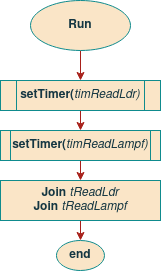
\includegraphics[width=.3\textwidth]{09sw_specification/LS/clocalsystem/run}
	\caption{Flowchart: CLocalSystem Run method.}
	\label{fig:CLocalSystemRun}
\end{figure}

%******************************
In figure \ref{fig:CLocalSystemtLoraRecv} is presented the task responsible for receiving a message from the gateway, via LoRa communication, parse it and execute the respective command.

\begin{figure}[H]
	\centering
	%	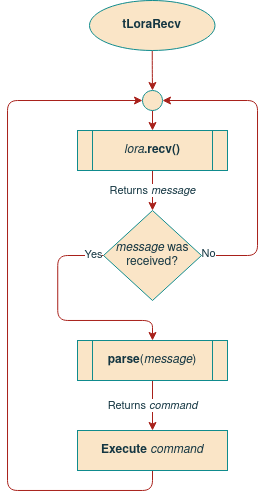
\includegraphics[width=.3\textwidth]{09sw_specification/LS/clocalsystem/tlorarecv}
	\caption{Flowchart: CLocalSystem tLoraRecv method.}
	\label{fig:CLocalSystemtLoraRecv}
\end{figure}

%******************************
In figure \ref{fig:CLocalSystemtRecvSensors} is presented the task responsible for receiving messages from the sensors daemon, via message queue. When there are no messages to read from the message queue, the task goes to sleep and is awaken when \textit{condRecvSensors} is notified. This happens in the \textit{sigHandler}, presented in figure \ref{fig:CLocalSystemsigHandler}, which is the signal handler for the main process, being this in charge of signaling the condition variable \textit{condRecvSensors} when a \textit{SIGUSR1} signal is catched.

\begin{figure}[H]
	\centering
	%	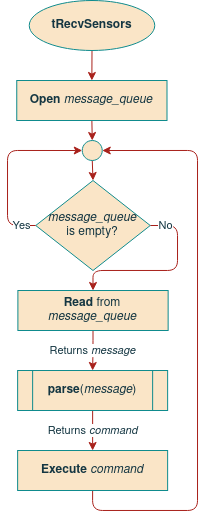
\includegraphics[width=.3\textwidth]{09sw_specification/LS/clocalsystem/trecvsensors}
	\caption{Flowchart: CLocalSystem tRecvSensors method.}
	\label{fig:CLocalSystemtRecvSensors}
\end{figure}

\begin{figure}[H]
	\centering
	%	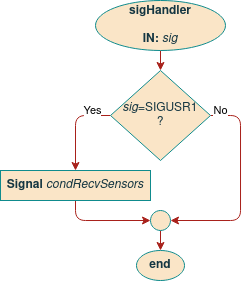
\includegraphics[width=.3\textwidth]{09sw_specification/LS/clocalsystem/sighandler}
	\caption{Flowchart: CLocalSystem sigHandler method.}
	\label{fig:CLocalSystemsigHandler}
\end{figure}

%******************************
This task, figure \ref{fig:CLocalSystemtParkDetection}, is responsible for using the \textit{camera} object, from \textit{CCamera}, and the \textit{park} object, from \textit{CParkDetection}, in order to capture image frames and process them, calculating the number of available spaces in the parking detected. This task is periodically awaken by the use of a timer, signaling the condition variable \textit{condCamFrame}.

%In the image processing part of the thread, if there aren't parking spots coordinates stored, then it is necessary to search for parking spots. After that, one can detect cars using the pre-trained model and the function \textit{detectCars} that detects cars in the image. 
%
%If the coordinates of a detected car matches the coordinates of the parking spot, then one can assume that the parking spot is occupied. If the parking spot status has changed, then it is necessary to send this to the remote system, using the LoRa communication module. In figure \ref{fig:}, is shown the thread \textit{tCamera} flowchart.


\begin{figure}[H]
	\centering
	%	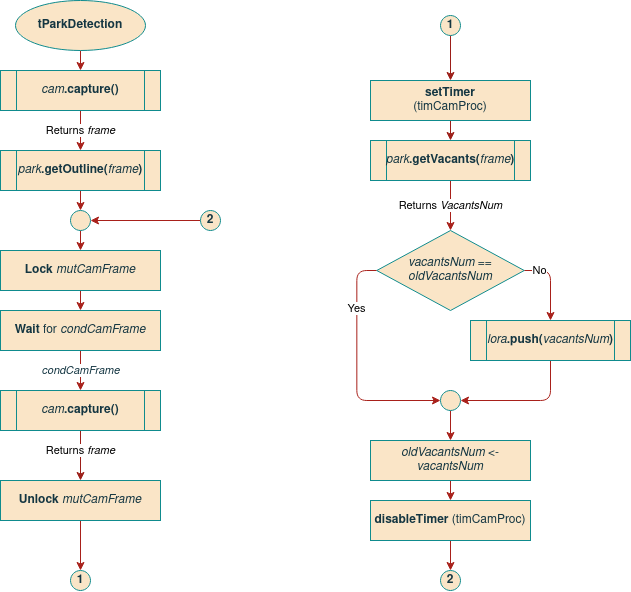
\includegraphics[width=.3\textwidth]{09sw_specification/LS/clocalsystem/tparkdetection}
	\caption{Flowchart: CLocalSystem tParkDetection method.}
	\label{fig:CLocalSystemtParkDetection}
\end{figure}

%**********************************************************
\clearpage
\myparagraph{CSensors Methods}

As in the previous class, the class constructor and the \textit{run()} method serves similar purposes, therefore, one has no need to specify them.\linebreak

In figure \ref{fig:CSensorstreadldr} is shown the task responsible for reading luminosity sensors from the LDR sensor. If there is a change in the luminosity state, a command is sent to the main process, using \textit{sendCmd(cmd)} method.

\begin{figure}[H]
	\centering
	%	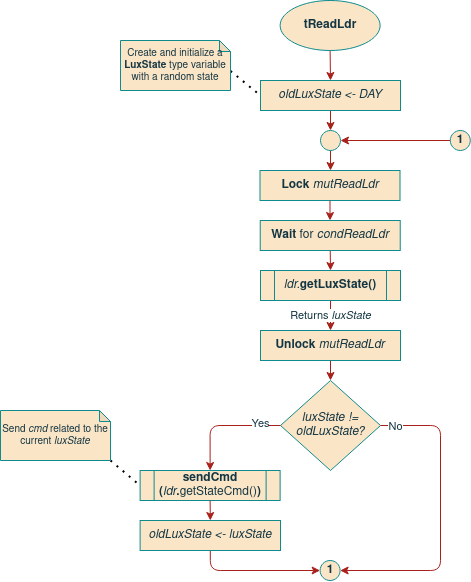
\includegraphics[width=.3\textwidth]{09sw_specification/LS/csensors/treadldr}
	\caption{Flowchart: CSensors tReadLdr method.}
	\label{fig:CSensorstreadldr}
\end{figure}

%******************************
aaaaaaaaaaaaaaa

\begin{figure}[H]
	\centering
	%	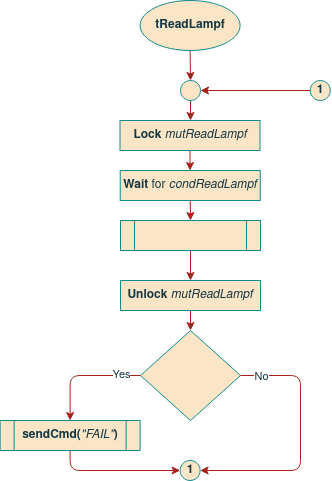
\includegraphics[width=.3\textwidth]{09sw_specification/LS/csensors/treadlampf}
	\caption{Flowchart: CSensors tReadLampf method.}
	\label{fig:CSensorstreadlampf}
\end{figure}

%******************************
The method \textit{sendCmd}, shown in figure \ref{fig:CSensorssendcmd}, is responsible for sending a string, \textit{cmd}, to the message queue, \textit{msgqSensors}. After that, it sends a signal, \textit{SIGUSR1}, to the process \textit{mainPID}, which is the main process PID.

\begin{figure}[H]
	\centering
	%	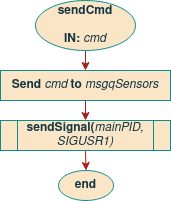
\includegraphics[width=.3\textwidth]{09sw_specification/LS/csensors/sendcmd}
	\caption{Flowchart: CSensors sendCmd method.}
	\label{fig:CSensorssendcmd}
\end{figure}

%******************************
The method \textit{PirISR}, is executed when there is motion detected, sending the \textit{"ON"} command to the main process.

\begin{figure}[H]
	\centering
	%	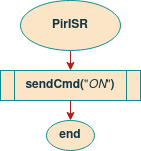
\includegraphics[width=.3\textwidth]{09sw_specification/LS/csensors/pirisr}
	\caption{Flowchart: CSensors PirISR method.}
	\label{fig:CSensorspirisr}
\end{figure}

%**********************************************************
\clearpage
\myparagraph{CCommunication Methods}

The class constructor is shown in figure \ref{fig:CCommunicationConstructor}. This is responsible for initializing all synchronization tools and private variables used.

\begin{figure}[H]
	\centering
%	\includegraphics[width=.3\textwidth]{09sw_specification/LS/ccommunication/constructor}
	\caption{Flowchart: CCommunication constructor.}
	\label{fig:CCommunicationConstructor}
\end{figure}

%******************************
To send a message, this class has a built-in thread, \textit{tSend} that can be created using \textit{init(tprio)}, which expects a priority for the thread, \textit{tprio}, as shown in figure \ref{fig:CCommunicationinit}.

\begin{figure}[H]
	\centering
	%	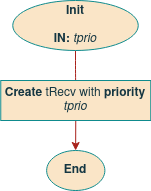
\includegraphics[width=.25\textwidth]{09sw_specification/LS/ccommunication/init}
	\caption{Flowchart: CCommunication Init method.}
	\label{fig:CCommunicationinit}
\end{figure}

%******************************
A message can be put in the waiting list to be sent through the use of \textit{push(msg)}, as shown in figure \ref{fig:CCommunicationPush}. This function is responsible for adding a new message, \textit{msg}, to the \textit{TxMsgs} vector, and signal the condition variable \textit{condSend}, for the thread \textit{tSend} to send the message.

\begin{figure}[H]
	\centering
%	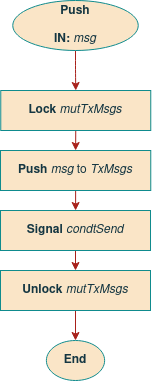
\includegraphics[width=.3\textwidth]{09sw_specification/LS/ccommunication/push}
	\caption{Flowchart: CCommunication Push method.}
	\label{fig:CCommunicationPush}
\end{figure}

%******************************
This thread, \textit{tSend} presented in figure \ref{fig:CCommunicationtsend}, is responsible for sending queued messages to the gateway, using LoRa communication. A conditional variable is used to wake this thread when there is a new message available to be sent.

When the queue \textit{TxMsgs} is empty, the task goes to sleep, waiting for the condition variable \textit{condSend} to notify this task. After this, the mutex \textit{mutComms} is used to protect the communication. Then, a message is popped from the messages queue, and sent to the gateway using the method \textit{Send}, shown in figure \ref{fig:CCommunicationsend}. This continues to happen until the \textit{TxMsgs} queue gets empty.

\begin{figure}[H]
	\centering
%	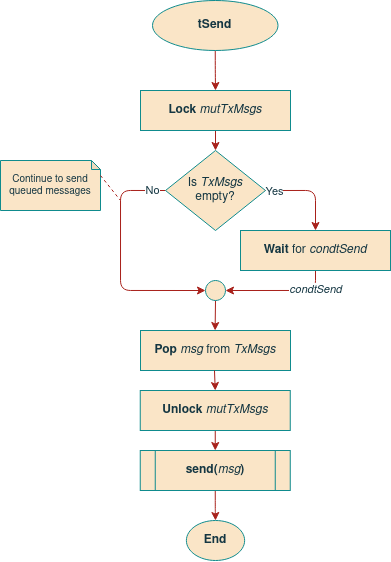
\includegraphics[width=.65\textwidth]{09sw_specification/LS/ccommunication/tsend}
	\caption{Flowchart: CCommunication tSend thread.}
	\label{fig:CCommunicationtsend}
\end{figure}

\begin{figure}[H]
	\centering
%	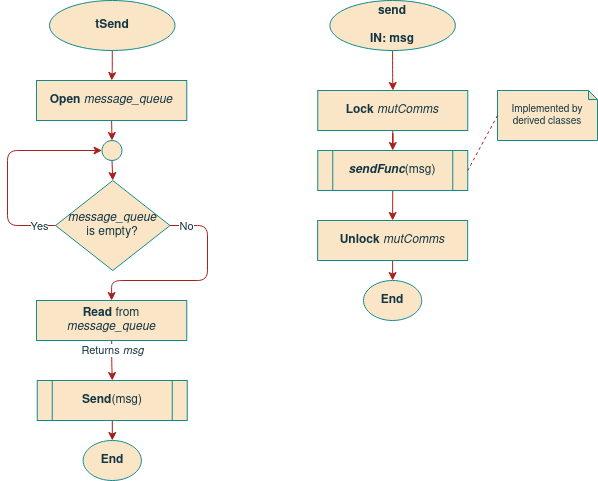
\includegraphics[width=.55\textwidth]{09sw_specification/LS/ccommunication/send}
	\caption{Flowchart: CCommunication Send method.}
	\label{fig:CCommunicationsend}
\end{figure}

%******************************
There is also another method, \textit{recv()}, that receives a message from the gateway, in a non blocking mode, making use of task synchronization tools to ensure that sending and receiving don't occur at the same time. This function should be used continuously if one doesn't want to miss any communication. This method is presented in figure \ref{fig:CCommunicationrecv}.

\begin{figure}[H]
	\centering
%	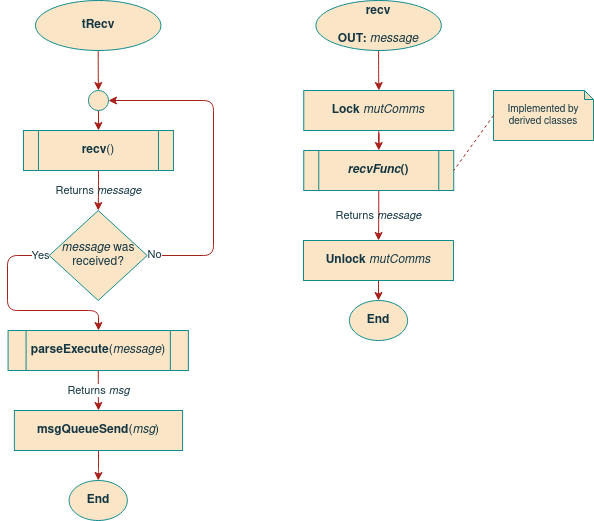
\includegraphics[width=.5\textwidth]{09sw_specification/LS/ccommunication/recv}
	\caption{Flowchart: CCommunication Recv method.}
	\label{fig:CCommunicationrecv}
\end{figure}

%**********************************************************
\clearpage
\myparagraph{CLoraComm Methods}

An object can be created through the use of the constructor, as shown in figure \ref{fig:LoraComm}.
This starts by initializing the LoRa communication, defining the pins connected to the module and the frequency in which the device chosen previously operates, which is 433~MHz. At the end, all private members are also initialized.

\begin{figure}[H]
	\centering
%	\includegraphics[width=.6\textwidth]{09sw_specification/LS/cloracomm/constructor}
	\caption{Flowchart: CLoraComm constructor.}
	\label{fig:LoraComm}
\end{figure}

\begin{figure}[H]
	\centering
	%	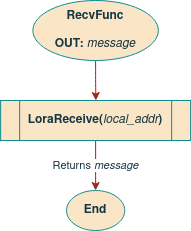
\includegraphics[width=.6\textwidth]{09sw_specification/LS/cloracomm/recvfunc}
	\caption{Flowchart: CLoraComm recvFunc method.}
	\label{fig:CLoraCommrecvfunc}
\end{figure}

\begin{figure}[H]
	\centering
	%	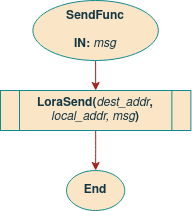
\includegraphics[width=.6\textwidth]{09sw_specification/LS/cloracomm/sendfunc}
	\caption{Flowchart: CLoraComm sendFunc method.}
	\label{fig:CLoraCommsendfunc}
\end{figure}


%**********************************************************
\clearpage
\myparagraph{CLamp Methods}

%******************************
%This function, presented in figure \ref{fig:flow_setbrightness}, is responsible for changing the PWM associated with the lamp, which is directly related to its brightness. Through \textit{setPWM(lux)} one can change the current lamp PWM to \textit{lux} value, being this an integer between 0 to 100. When the PWM is maximum, a timer is started that defines how much time the lamp is ON, \textit{LAMP\_ON\_TIMEOUT} in seconds, if there isn't another call of this function.

\begin{figure}[H]
	\centering	
	%	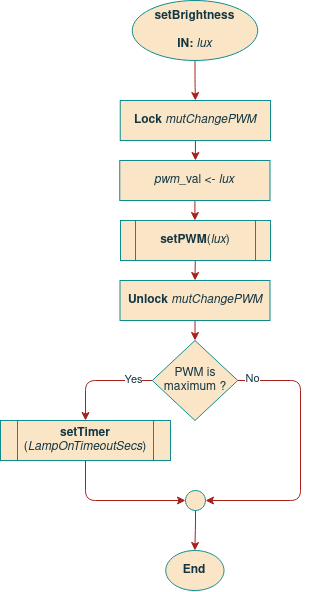
\includegraphics[width=.6\textwidth]{09sw_specification/clamp/setbrightness}
	\caption{Flowchart: CLamp setBrightness method.}
	\label{fig:CLampsetBrightness}
\end{figure}

%**********************************************************
\clearpage
\myparagraph{CParkDetection Methods}


%******************************
This function, represented in figure \ref{fig:CParkDetectiongetoutline}, is used to process the image captured by the camera in order to detect the parking spots outline. This is done using the algorithm defined previously in the section \ref{section:imageProc}, and starts by converting the frame to a grey scale image, apply the canny edge filter to highlight the edges of the image captured. After having the edges, one can select only the vertical and horizontal straight lines and intersect them, storing the intersection points, that are the parking spot coordinates.

\begin{figure}[H]
	\centering			
	%	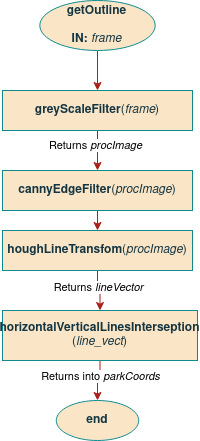
\includegraphics[width=.5\textwidth]{09sw_specification/cparkdetection/getoutline}
	\caption{Flowchart: CParkDetection getOutline method.}
	\label{fig:CParkDetectiongetoutline}
\end{figure}

%**********************************************************
\clearpage
\myparagraph{CLdr Methods}
%getLuxState
%getStateCmd

%\myparagraph{getLuxState}
%The ambient light sensor, LDR, is used to determine when is time to turn on the lights, that is, when is night time and interfaces with the Raspberry Pi through I2C protocol communication. As the sun set or the sun rise is a relatively long time process, there's no need to keep checking the sensor output value all the time, so one can define a period to get the sensor value, \textit{LDR\_TIM}, that can be 10 minutes. In figure \ref{fig:ldr_isr} is shown the LDR sensor interrupt service routine, triggered by the timer overflow. When the timer period elapses, the illuminance value is calculated by the sensor. If this value is lower than the threshold value defined as good luminosity illuminance, GOOD\_LIGHT\_LUX, then the auxiliary variable, \textit{lightCon} is setted to high. In the next step, if the \textit{oldLightCon} variable (stores the last ambient light condition) is not equal to the auxiliary variable, then it is needed to change the \textit{oldLightCon} variable and send message to the process that controls the lamp PWM, through message queue. 

\begin{figure}[H]
	\centering
	%	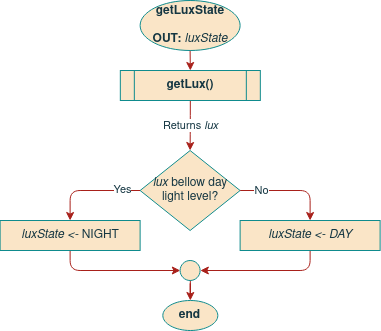
\includegraphics[width=.7\textwidth]{09sw_specification/LS/cldr/getluxstate}
	\caption{Flowchart: CLdr getLuxState method.}
	\label{fig:CLdrgetLuxState}
\end{figure}


%**********************************************************
\clearpage

\begin{itemize}
%	\item Lamp Max: the lamp brightness must be at its maximum (PWM=100);
	\item Lamp Min: the lamp must be at minimum bright level (PWM = \textit{MIN\_BRIGHT\_PWM});
	\item Lamp OFF: the lamp must be OFF (PWM=0);
	\item Lamp Fail: the lamp must be OFF, since there was a failure detected on the lamp.
\end{itemize}

